\iflanguage{ngerman}
{\chapter{Ergebnisse}}
{\chapter{Results}}

\label{sec:results}
Im Folgenden werden die Ergebnisse der zuvor beschriebenen Umsetzung Ausgewertet.
Dabei wird insbesondere auf die, mit der Funktionalität des Plugins erreichten Ziele in der Aufgabenstellung eingegangen.
Anschließend gibt es eine kurze Performance-Evaluation.

\section{Software-Interface}
Hier wird kurz beschrieben wie man die Funktionen des Plugins auch außerhalb des Demo-Interfaces nutzen kann.
\par
Durch das befüllen der Vektoren 'graph\_data' und 'graph\_param' in der Hauptklasse, können beliebige Graphdaten geladen werden.
Mit 'graph\_param' lässt sich zudem die Färbung und relative Skalierung der Graphen zueinander anpassen.
Als Referenz kann die Funktion 'gen\_graph\_data' genutzt werden, die die Demo-Daten generiert und damit die Vektoren befüllt.
\par
Der Integer 'graph\_count' stellt die Anzahl der Graphen dar, die aus den Vektoren tatsächlich dargestellt werden.
Normalerweise wäre diese Anzahl genau die Zahl an Graphen die gerade in den Vektoren geladen sind.
\par
Der 'segment\_type' gibt an, welcher Segmenttyp genutzt wird, entweder 'LINE\_SEGMENT' oder 'PARALLEL'.
Ohne weitere Modifikationen sollte möglichst nur der Typ 'LINE\_SEGMENT' genutzt werden, die Gründe werden in Abschnitt \ref{sec:line-parallel} erläutert.
\par
Sämtliche weitere Einstellungen können mit den Slidern im Demo-Interface ausprobiert werden.

\section{Nutzer-Interface}
Das Nutzer Interface des Plugins nutzt wie zuvor beschrieben das interne GUI-System des CGVF.
In Abbildung \ref{fig:ui} ist die Nutzeroberfläche einmal dargestellt.
Dieses Interface ist sehr rudimentär und dient eher zum Testen der verschiedenen Funktionalitäten, als der endgültigen Nutzung.
Es gibt Schalter zum aktivieren/deaktivieren von Tickmarks, dem Grid, den hervorgehobenen Hauptachsen, den Graphen und dem Hintergrund des Grids.
Zudem gibt es Slider für andere Einstellungen.
Die minimalen und maximalen Werte der Slider sind oft in einem 'Testbereich' gewählt, dass heißt viele Werte können auch außerhalb dieser Grenzen Liegen.
\begin{figure}[ht]
	\centering
	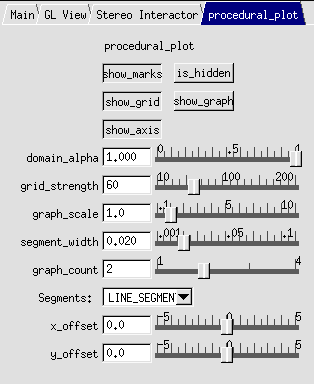
\includegraphics[width=0.3\textwidth]{fig/ui.png}
	\caption{Nutzer-Interface}
	\label{fig:ui}
\end{figure}
\FloatBarrier

\section{Graphen-Darstellung}
Die generelle Darstellung von ununterbrochenen Graphen funktioniert zuverlässig und gut bei der Nutzung von Liniensegmenten.
Ein Beispiel mit allen Testgraphen ist in Abbildung \ref{fig:all-graphs} zu sehen.
\begin{figure}[ht]
	\centering
	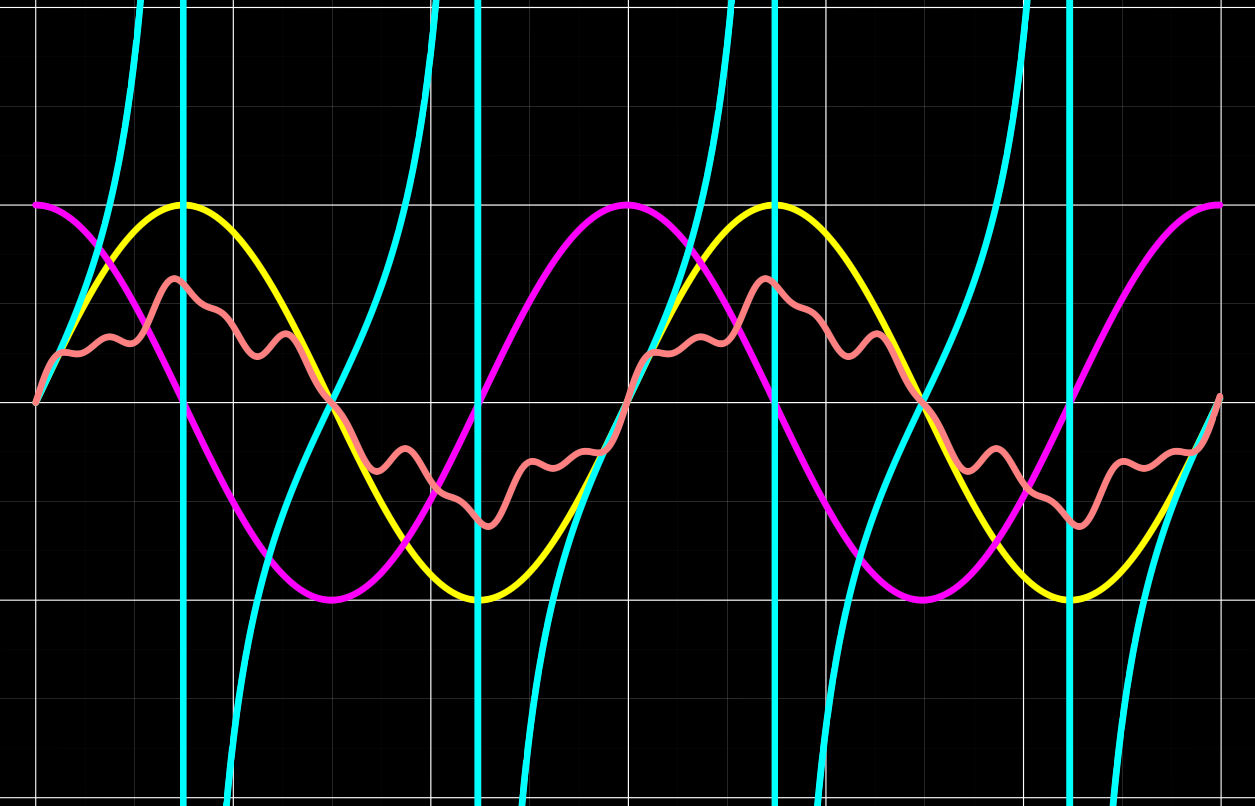
\includegraphics[width=0.6\textwidth]{fig/all-graphs.png}
	\caption{Test von vier Graphen mit Linien-Segmenten}
	\label{fig:all-graphs}
\end{figure}
\FloatBarrier
\subsection{Liniensegmente und Parallelogrammsegmente}
\label{sec:line-parallel}
Auch wenn bei der Umsetzung zwei verschiedene Segmenttypen zum Einsatz kamen, gibt es de facto nur einen Typ der wirklich funktioniert.
Nur die Liniensegmente schaffen eine einfache und problemfreie Darstellung.
Im Folgenden wird auf die zwei größten Probleme mit der Alternative, den Parallelogrammsegmenten eingegangen.
\par
Zunächst das Problem mit der gleichmäßigen Linienstärke.
In den Abbildungen \ref{fig:linie-graph2} und \ref{fig:parallelogramm-graph2} werden jeweils die Sinus- und Kosinus-Kurven gezeigt.
Bei der Nutzung von Liniensegmenten sieht man Graphen mit gleichmäßiger Zeichenstärke, doch bei Nutzung von Parallelogrammsegmenten sieht man eine ungleichmäßige Stärke.
Dass kommt daher, dass sich ein Parallelogramm bei starkem Anstieg oder Abstieg, vertikal verzerrt.
Zudem müssen die Seitenflächen an den Übergängen zu Nachbarsegmenten gleich zu denen der Nachbarn sein, damit der Graph keine Stufen hat.
Ich habe während der Bearbeitungszeit keine Lösung dafür gefunden und bin mir auch nicht sicher ob es eine (effiziente)Lösung gibt.
\begin{figure}[ht]
	\centering
	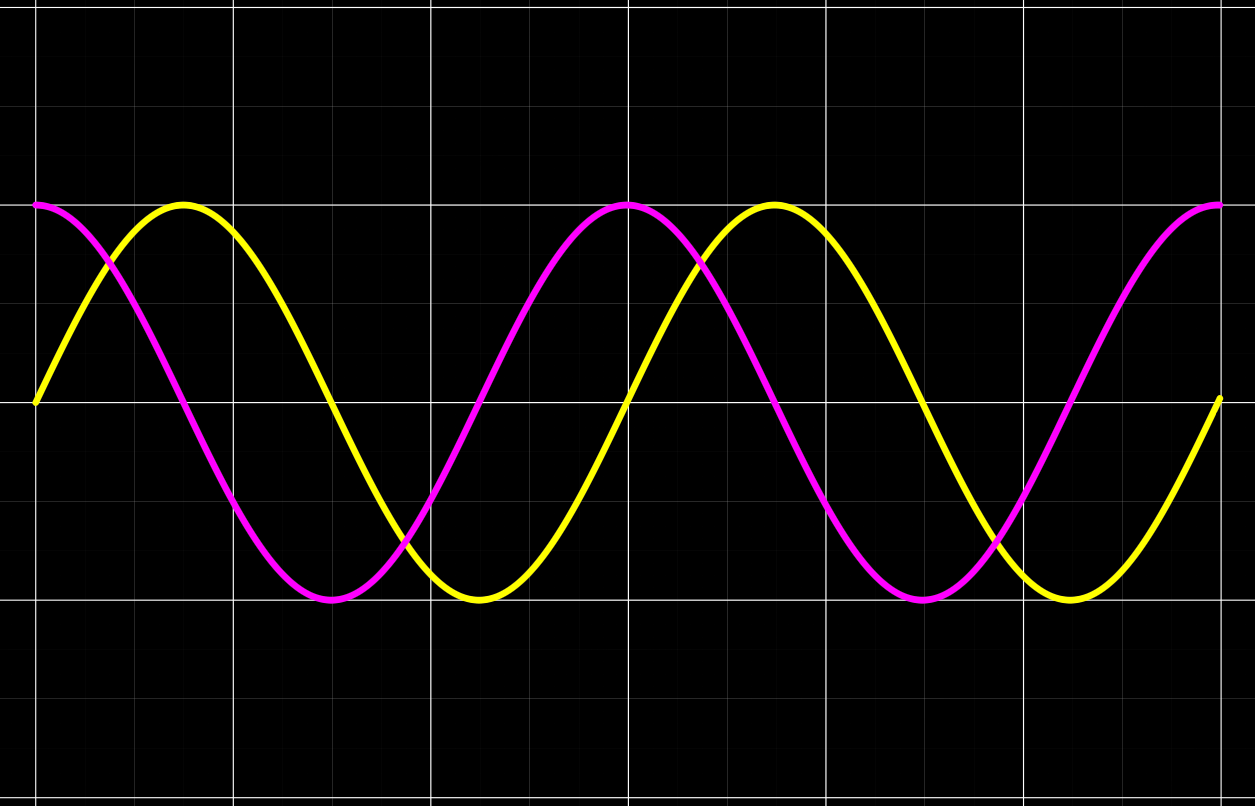
\includegraphics[width=0.6\textwidth]{fig/linie-graph2.png}
	\caption{Test von zwei Graphen mit Linien-Segmenten}
	\label{fig:linie-graph2}
\end{figure}
\FloatBarrier
\begin{figure}[ht]
	\centering
	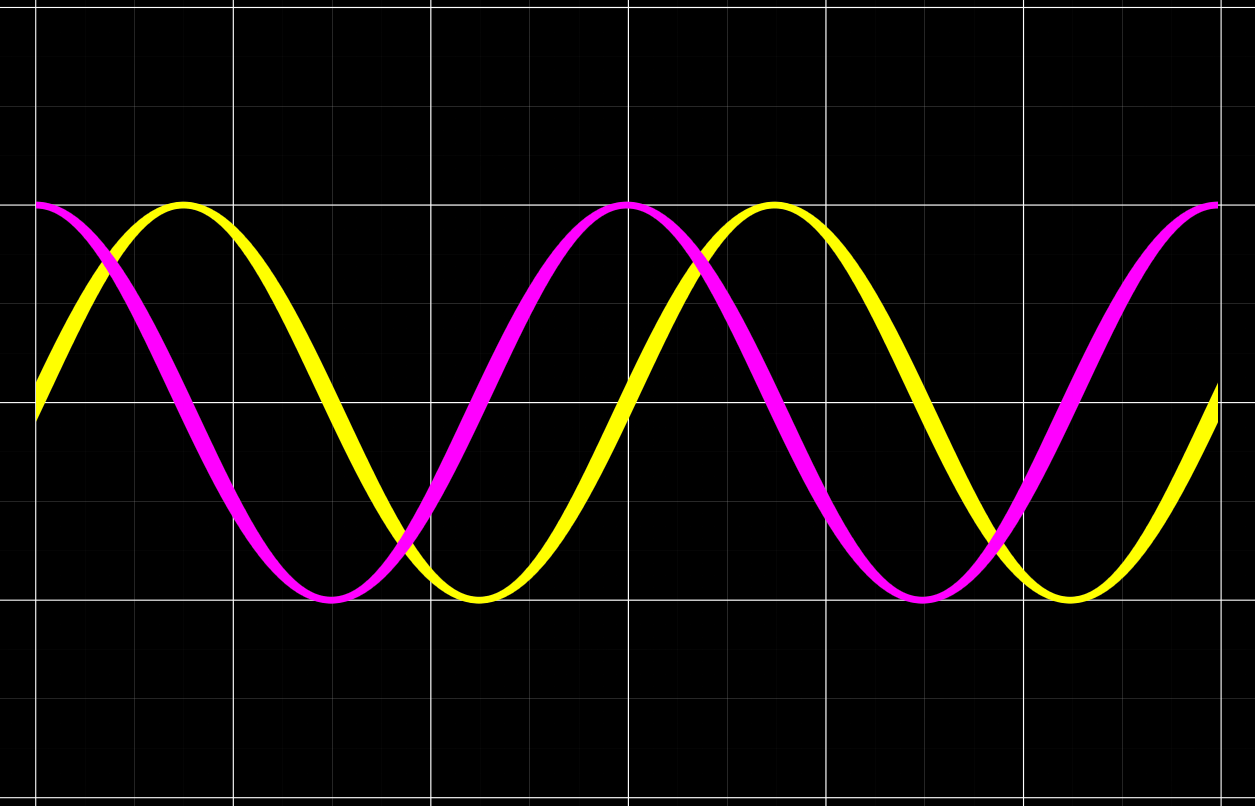
\includegraphics[width=0.6\textwidth]{fig/parallelogramm-graph2.png}
	\caption{Test von zwei Graphen mit Parallelogramm-Segmenten}
	\label{fig:parallelogramm-graph2}
\end{figure}
\FloatBarrier
Ein weiteres Problem mit den Parallelogrammsegmenten ist ein Fehler, der die Seitenflächen leicht voneinander abweichen lässt.
Das hat wahrscheinlich damit zu tun, dass eine Seite eine andere Höhe braucht als die Andere.
Mit diesem Fehler konnte Ich mich noch gar nicht auseinandersetzen, wollte ihn aber dennoch erwähnen.
Die Abbildung \ref{fig:parallelogramm-kante} und \ref{fig:linie-kante} zeigen deutlich das Problem und den Vergleich zur Nutzung der Liniensegmente.
\begin{figure}[ht]
	\centering
	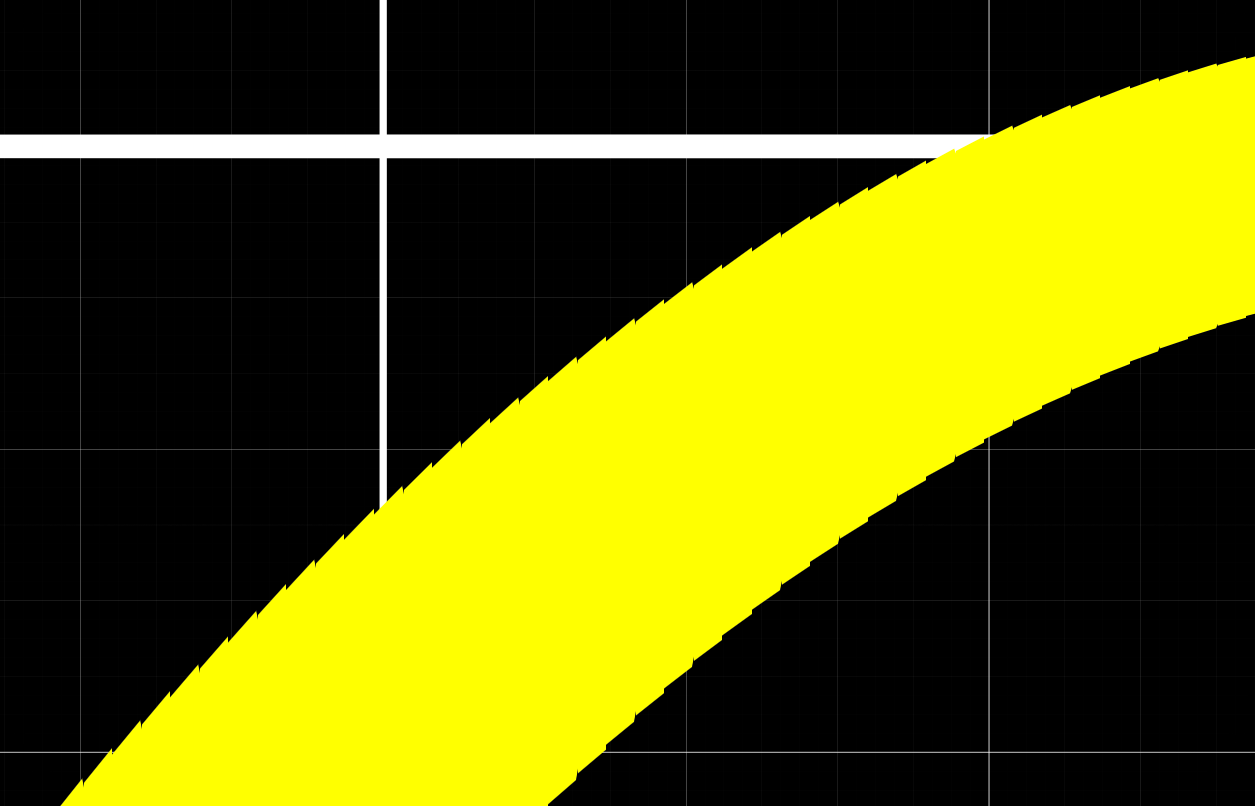
\includegraphics[width=0.6\textwidth]{fig/parallelogramm-kante.png}
	\caption{Parallelogramm-Segment vergrößert}
	\label{fig:parallelogramm-kante}
\end{figure}
\FloatBarrier
\begin{figure}[ht]
	\centering
	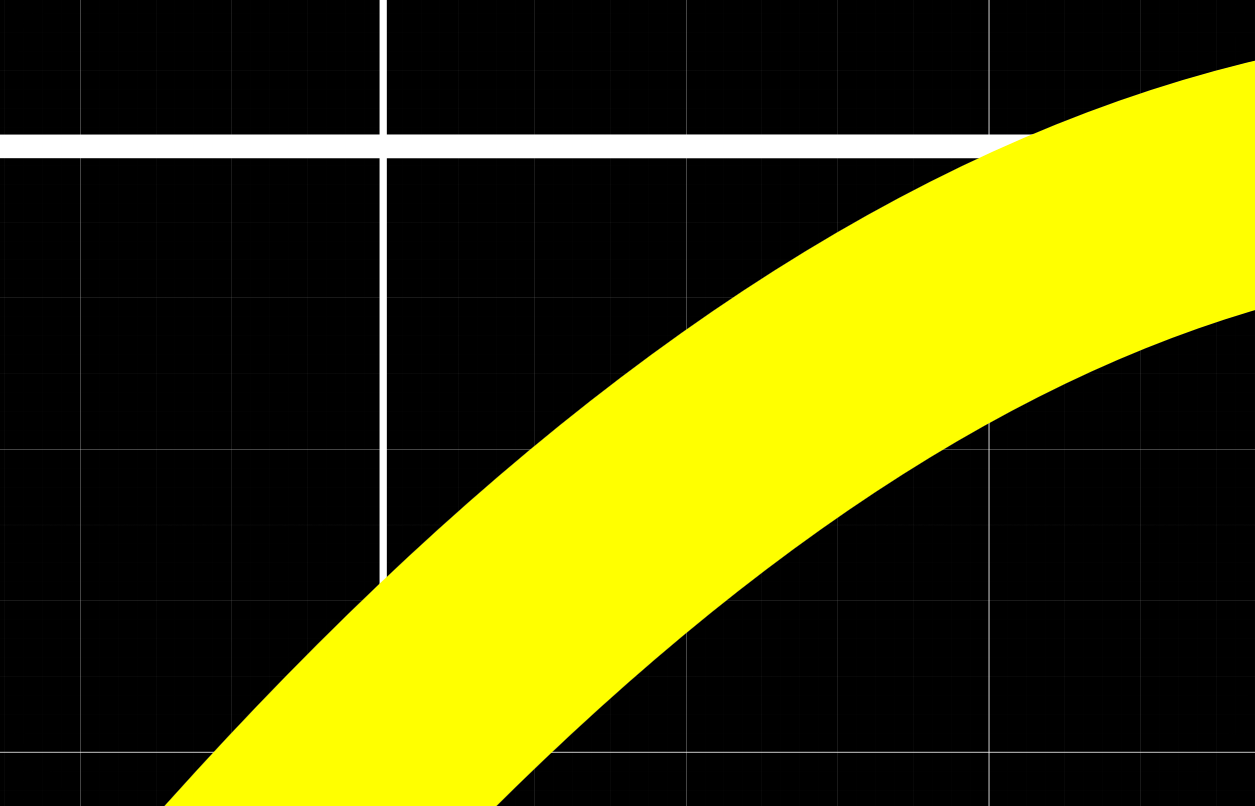
\includegraphics[width=0.6\textwidth]{fig/linie-kante.png}
	\caption{Linien-Segment vergrößert}
	\label{fig:linie-kante}
\end{figure}
\FloatBarrier

\section{Grid}
Das statische Grid als wichtigst Dekoration bei der Plot-Visualisierung funktioniert ohne Probleme und hat genau eine Unterteilung pro Achseneinheit.
Die Stärke des Grids kann angepasst werden und der Ursprung orientiert sich immer am Ursprung des Plot-Raums.
\par
Das dynamische Grid funktioniert zwar, ist aber noch ein Prototyp.
Wie in Abbildung \ref{fig:grid} zu sehen, werden die Grid-Linien dünner mit feinerer Auflösung.
\begin{figure}[ht]
	\centering
	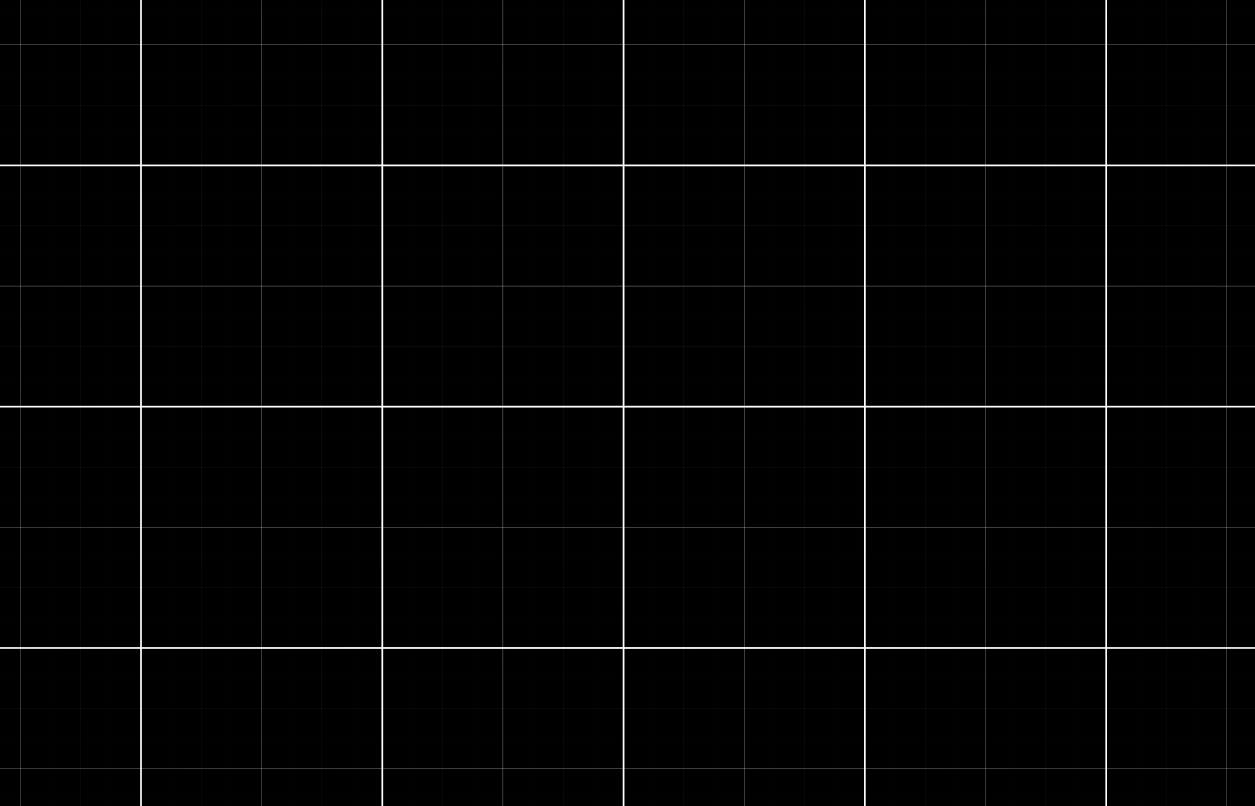
\includegraphics[width=0.6\textwidth]{fig/grid.png}
	\caption{Dynamisches Grid}
	\label{fig:grid}
\end{figure}
\FloatBarrier
Die Sichtbarkeit der Ebenen hängt von der Position der Kamera im 3D-Raum ab.
Ist die Kamera näher dran, sind auch mehr Linien sichtbar.
Die maximale Anzahl der Ebenen ist auf momentan auf 9 beschränkt und Ebene mit der gröbsten Auflösung ist immer das statische Grid, mit einer Unterteilung pro Achseneinheit.
Aufgrund dieser Einschränkungen betrachte Ich es als Prototyp.

\section{Andere Dekorationen}


\section{Performance}
Zuletzt in der Auswertung wird die Performance im Bezug auf das Darstellen von durchgängigen Graphen im Plot evaluiert.


\subsection{SDF}
Die beiden SDFs, die für die Graphensegmente genutzt werden stammen beide von Inigo Quilez \cite{Inigo} und soweit Ich dass beurteilen kann, sind Beide optimal und Sie lassen sich nicht weiter vereinfachen.
Das von mir testweise Erstellte 'sdf\_parallelogram\_segment' ist spürbar Langsamer als die Implementation von Quilez, weswegen früh klar war, dass es sich nicht lohnt eigene SDF-Implementationen weiter zu erforschen.

\subsection{Binärsuche bei Segmenten}
Der größte Performance-Faktor beim Darstellen der Graphen ist die 'quasi' Binärsuche nach relevanten Segmenten.
Meine Implementation der Suche ist sicherlich nicht optimal, funktioniert aber zuverlässig und ist erheblich schneller als das Verzichten auf eine Suchfunktion.
\par
Bei Parallelogrammsegmenten ist die Suchzeit immer in der Klasse von $O(\log{}n)$.
Bei den Liniensegmenten gibt es eine zusätzliche Abhängigkeit von der Linienstärke.
Das kommt daher, dass sich die Liniensegmente an den Messpunkten in den Graph-Daten überlappen.
Diese Überlappung wird größer, sobald die Linienstärke wächst.
Ist die Linienstärke groß genug, kann ein Segmentrand sogar ein anderes Segment komplett in der X-Richtung überdecken.
Da die anderen Segmente nicht auf der gesamten Fläche überdeckt werden, entstehen visuelle Artefakte wenn man überdeckte Segmente einfach weglässt.
Daher muss berechnet werden, wie viele Segmente bei der Momentanen Linienstärke überlappt werden können; mehr dazu in Abschnitt \ref{sec:binary}.
Bei jedem Schritt in der Suche muss jetzt in beide Richtungen geprüft werden, ob nicht noch Andere Segmente überlappen könnten.
Bestenfalls erreicht die Binärsuche dabei eine Suchzeit in der Klasse von $O(3*\log{}n)$, da direkte Nachbarsegmente immer überlappen.
Schlimmstenfalls kommt es zu einer Suchzeit in der Klasse von $O(n^2)$.
Dieser schlimmste Fall tritt aber in der realen Nutzung praktisch nie auf, da man mit einer so großen Linienstärke nichts mehr vom Graphen erkennen würde.
Daher betrachte Ich diese Abhängigkeit nicht als ein großes Problem. 

%\subsection{Referenzwerte}